\documentclass[11pt,a4paper]{article}

\usepackage[utf8]{inputenc}
\usepackage[T1]{fontenc}
\usepackage{graphicx}
\usepackage{float}
\usepackage{booktabs}
\usepackage{geometry}
\usepackage{setspace}
\usepackage{fancyhdr}
\usepackage{caption}
\usepackage{amsmath}
\usepackage{xcolor}
\usepackage{hyperref}

\geometry{a4paper, margin=2.5cm}
\setstretch{1.1}
\hypersetup{colorlinks=true, linkcolor=black, urlcolor=blue, citecolor=black}

\pagestyle{fancy}
\fancyhf{}
\fancyhead[L]{Individual Project Report}
\fancyhead[R]{Antidepressant Patient Rates}
\fancyfoot[C]{\thepage}
\setlength{\headheight}{14pt}


\title{District Unemployment and Antidepressant Patient Rates\\in New Zealand, 2021--2025}
\author{Jessica Saucedo 300666254\\[0.3em]
\small DATA301 Individual Project Report, Victoria University of Wellington\\\small Phase 1 group members: Nam Bui, Tianyi Xu, Zion Swinburne}
\date{\tbc{25 Octuber 2026}}

\begin{document}
\maketitle
% =========================================================
\section *{Executive Summary}

This project looks at whether health districts in New Zealand with higher levels of unemployment have different numbers of people on antidepressants. I've merged Health NZ pharmaceutical data with the 2023 Census data for the 19 health districts from 2021 to 2025. For each district and year I've calculated the antidepressant patient rate (the number of people who received at least one initial antidepressant dispensing in that year, for every 1,000 residents).

Districts with higher levels of unemployment had lower antidepressant patient rates. After allowing for the proportion of residents aged 30- 64 and for the year, each additional percentage point of unemployment was associated with around 12.5 fewer patients per 1,000 (95\% CI: 7.3 to 17.7 fewer; p < 0.001). To put that in some context, the model suggests that a district with 6.1\% unemployment (the highest) would have around 43 fewer patients per 1,000 than a district with 2.7\% unemployment (the lowest), all other things being equal. On average the rates were increasing by around 2.3 patients per 1000 per year (95\% CI: 1.8 to 2.8). Other sensible model specifications (including one that omitted the district with the lowest rate) all came to the same conclusion with estimates ranging from 10.4 to 15.1 fewer patients per 1,000.

This is a pattern across the districts. It doesn't suggest that unemployment leads to people using fewer antidepressants. Antidepressant dispensing is going to be determined by access to GPs and prescribing practice as much as it is by health need so a lower rate shouldn't be interpreted as lower need. With just 19 districts and the Census data from a single year (2023) the estimates are very uncertain.

\newpage

% =========================================================
\section{Background}

Antidepressants are one of the most commonly prescribed medicines in New Zealand. In our Phase 1 group analysis they were the 9th largest of the 127 medicine groups in terms of number of patients (2021 to 2025). The dispensing data are published by health district so they enable antidepressant use to be compared across different parts of the country. Antidepressants are also prescribed for other conditions and Health New Zealand makes it clear that a therapeutic group does not equate to a diagnosis \cite{hnz}. Dispensing is therefore used as a measure of medicine use rather than a measure of the number of people with a mental health condition.

Unemployment is generally linked to worse mental health \cite{mh}. One would therefore anticipate higher levels of antidepressant use in areas of higher unemployment. The direction of the association at a district level is however not at all obvious in advance as dispensing will also be influenced by whether people can get to a prescriber, how conditions are diagnosed and of course prescribing practice.

In Phase 1 we looked at the number of pharmaceutical patients across medicine groups, years and districts, adjusted for population and then compared that with the Census variables. That initial exploration was based on the raw Census counts (which essentially just tell you how big the district is). In this report I'm concentrating on one demographic variable (unemployment) and using percentages so that the size of the district doesn't dominate the comparison.

The question for this report is: Is the district unemployment rate associated with the antidepressant patient rate (patients per 1,000 residents), allowing for the age structure of the district and the year? The null hypothesis is that the effect of unemployment is zero. The alternative is that it is not zero. 


% =========================================================
\section{Data Description}

\subsection{Key definitions}
An \emph{initial dispensing}  is the first time a prescription item is dispensed (i.e. an item dispensed all at once), repeat dispensings of the same item are excluded \cite{hnz}. The number of patients is the number of different people (identified by their NHI number) who received at least one initial dispensing of the medicine group in the district during the year \cite{hnz}. People who only received repeat dispensings of an existing prescription that year are not included. A person with several initial dispensings in a year is counted only once and the same person can be in more than one year. The number of dispensings is the number of initial dispensings (i.e. it counts each event), so it will be greater than the number of patients if a person has more than one initial dispensing. This report uses the number of patients as it is a count of people and is less susceptible than dispensing counts to variation in the frequency with which a medicine is dispensed \cite{hnz}. Health New Zealand also recommend that patient counts should not be aggregated across different medicines as people will be prescribed more than one medicine in a year \cite{hnz}. This report therefore uses a single medicine group. The patient rate is the number of patients per 1,000 residents in the district.

\subsection{Pharmaceutical data}
Pharmaceutical data sourced from the Health New Zealand Pharmaceutical Data web tool \cite{hnz}. This tool provides a summary of community dispensed medicines that are funded by the New Zealand Government (so non subsidised medicines are not included). Each row is for one Therapeutic Group Level 2 medicine group, one health district and one year. The columns are: medicine group (categorical), district (categorical), year (2021 to 2025, numerical) and the counts (numerical). There are 127 medicine groups. This report is restricted to the “Antidepressants” group which has 20 districts and 5 years (100 rows). The national total row has been excluded as it is not a district. Each record is assigned to the district in which the patient lived at the time of dispensing (when their NHI number was recorded) and otherwise to the district which funds the pharmacy \cite{hnz}. \tbc{NHI completeness was 100\% for all antidepressant records so all records were assigned on the basis of place of residence.} 

\subsection{Census data}
Population and demographic data are from the 2023 Census \cite{census} and are provided at health district level. Two Census variables are used in the analysis. The unemployment rate is the percentage of the labour force who are unemployed, where the labour force is the number of people at full time work, part time work or unemployed:

\[
\text{unemployment rate} = \frac{\text{unemployed}}{\text{full time} + \text{part time} + \text{unemployed}} \times 100 .
\]

The \emph{age structure} variable is the \% of residents aged 30 to 64. The census counts are converted to percentages as the counts themselves are largely a reflection of the size of the district. The census population of each district is also the denominator for the patient rate.

\subsection{Combining the datasets}
Capital \& Coast and Hutt Valley were merged into a single district under the Pae Ora (Healthy Futures) Act 2022 \cite{paeora}. The 2023 Census uses the combined district but the pharma data still report the two separately, therefore I've added the patient numbers for each year for the two districts so that the districts matched. The census data has then been attached to each pharma record by matching on district name. This gives us 19 districts and 95 district - year observations.

\subsection{Completeness}
None of the 100 antidepressant patient counts were suppressed. In the broader dataset counts below 6 are reported as ``$<$6'' for privacy reasons and are not exact, but again none of the antidepressant counts in this instance were affected so no observations were removed. The Census variables didn't have missing values and no errors were found. The only thing is that the Census data is from 2023 and is used for all years so the changes in population and unemployment between 2021 and 2025 are not picked up. 

% =========================================================
\section{Ethics, Privacy and Security}

\subsection{Ethical considerations}
Antidepressant dispensing is health information on a sensitive subject. Even though the data
are summarised and cannot be used to identify individuals, the results could be misread (for example as a statement about the mental health of people in a particular district). I therefore only report on patterns across districts, do not rank or label any communities and treat dispensing as a measure of supply and access to medicine rather than as a measure of the amount of mental illness in a community. The data are at the district level so the results cannot be applied to individuals.

M\={a}ori data sovereignty is also relevant, because the data cover M\={a}ori communities. I avoid
deficit-based interpretations, and I do not draw any conclusions about any community from dispensing patterns alone.

\subsection{Privacy}
The pharma data are already aggregated and counts below 6 have been suppressed to protect small groups. I've kept that suppression and haven't attempted to reconstruct the suppressed values. I've used the Census data at health district level rather than at the smaller Statistical Area 1 level which would only cover 100 to 200 households and could in combination with other data allow for the identification of small groups (Stats NZ, 2026)\cite{sa1}.

\subsection{Data security}
Both datasets are public and contain no individual level information. The project files were stored in a public GitHub repo, the report was written in Overleaf shared by invitation and files and figures were shared via Google Docs. No further access controls (i.e. no encryption, no restricted sharing etc) were employed as no sensitive data were in fact used. If we had used any non public or more detailed data then I would have.

% =========================================================
\section{Exploratory Data Analysis}

Table~\ref{tab:summary} summarises the three variables used in the analysis across the 19 districts. The patient rate is the average for each district over 2021 to 2025.

\begin{table}[H]
\centering
\caption{Summary of the analysis variables across 19 health districts.}
\label{tab:summary}
\begin{tabular}{lrrr}
\toprule
\textbf{Variable} & \textbf{Minimum} & \textbf{Median} & \textbf{Maximum} \\
\midrule
Antidepressant patient rate (per 1,000 residents) & 83.7 & 134.2 & 149.0 \\
Unemployment rate (\%)                            & 2.7  & 4.3   & 6.1   \\
Residents aged 30--64 (\%)                        & 42.3 & 43.0  & 47.1  \\
\bottomrule
\end{tabular}
\end{table}

Figure~\ref{fig:bar} shows the patient rate in each district. The rates ranged from 83.7 patients per 1,000 in Counties Manukau to 149.0 in Canterbury (Wairarapa was very similar at 148.9) so the highest rate is about 1.8 times that of the lowest. As the rates are already population adjusted the differences are not due to the size of the district. The lowest rates were in Counties Manukau (83.7), Tair\={a}whiti (99.4) and Auckland (105.6).

\begin{figure}[H]
\centering
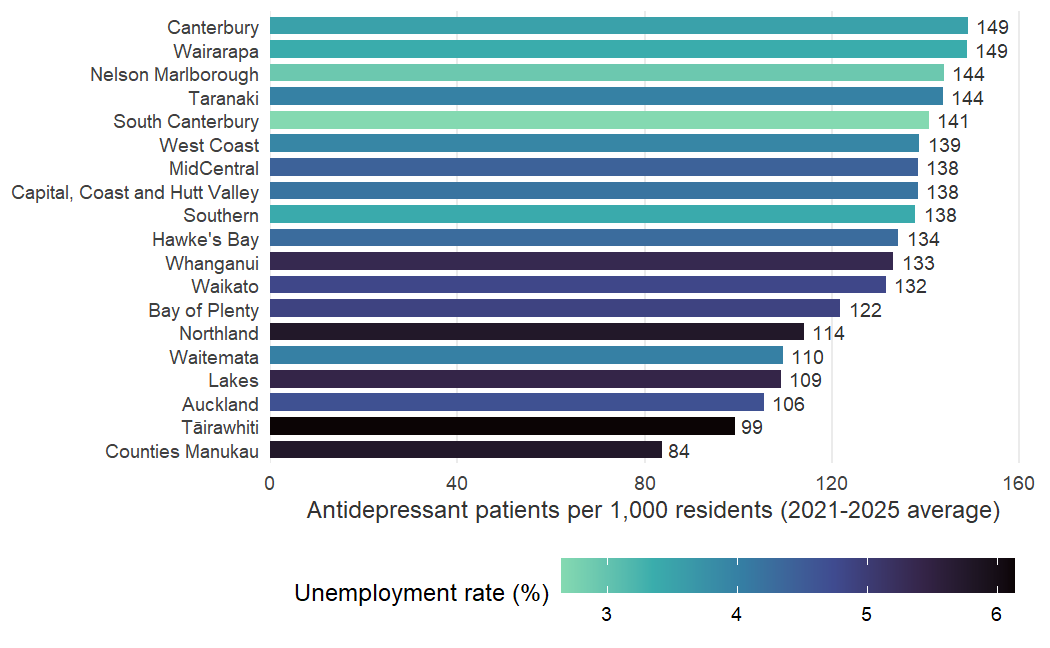
\includegraphics[width=0.75\textwidth]{district_rates_bar.png}
\caption{Average antidepressant patient rate by health district, 2021-2025. Bars are shaded by the district's unemployment rate (darker = higher), the number at the end of each bar is the rate.}
\label{fig:bar}
\end{figure}

Figure~\ref{fig:trend} shows the rates over time for the districts above the median unemployment rate (4.3\%, 9 districts) and for those at or below it (10 districts). Rates went up in both groups over time: from 133.2 to 143.9 per 1,000 in the lower unemployment districts and from 111.5 to 119.0 in the higher unemployment districts. The higher unemployment group remained lower in every year (by about 22 per 1,000 in 2021 and about 25 in 2025) so the gap between the groups is not a feature of any one year. The lines are the unweighted average of the districts in each group (so large and small districts are equally weighted).

\begin{figure}[H]
\centering
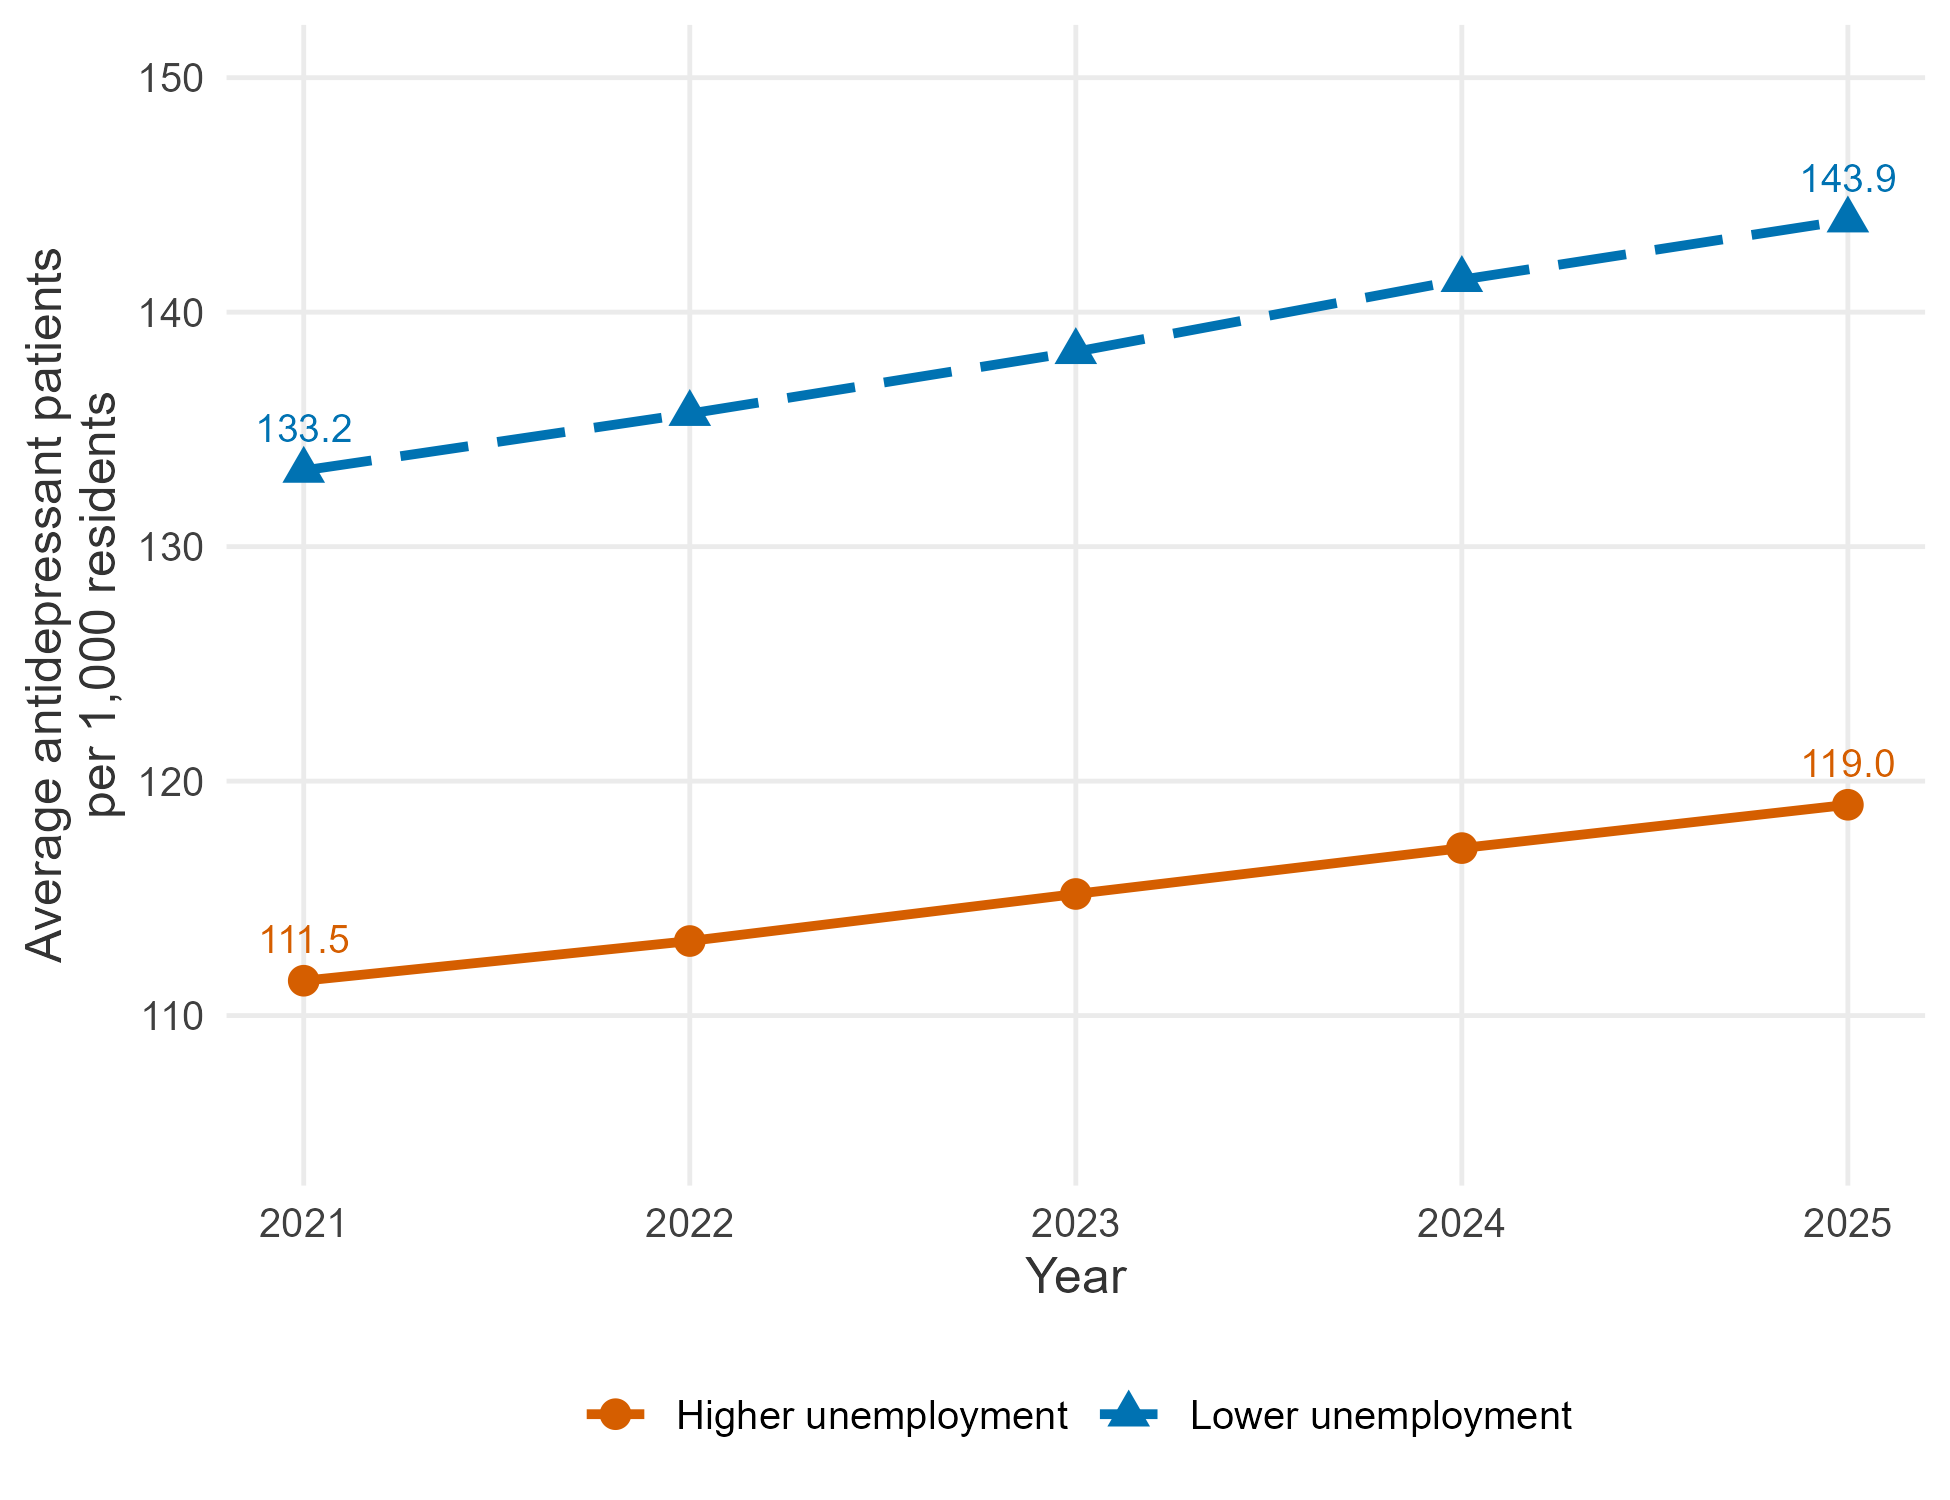
\includegraphics[width=0.7\textwidth]{trend_by_unemployment.png}
\caption{Average antidepressant patient rate by year for districts above and at or below the median unemployment rate (4.3\%).}
\label{fig:trend}
\end{figure}

Figure~\ref{fig:scatter} plots the average patient rate against it's unemployment rate for each district. The points slope downwards (districts with higher unemployment have lower rates). Counties Manukau (5.8\% unemployment) is well below the fitted line and therefore check that the result aren't driven by that one district. The fitted line is a simple one (no age or year in it) so it's just a first glance at the relationship which is tested in the next section. The two predictors in the model are not highly correlated with each other (correlation = $-0.17$) so their effects can be separated.

\begin{figure}[H]
\centering
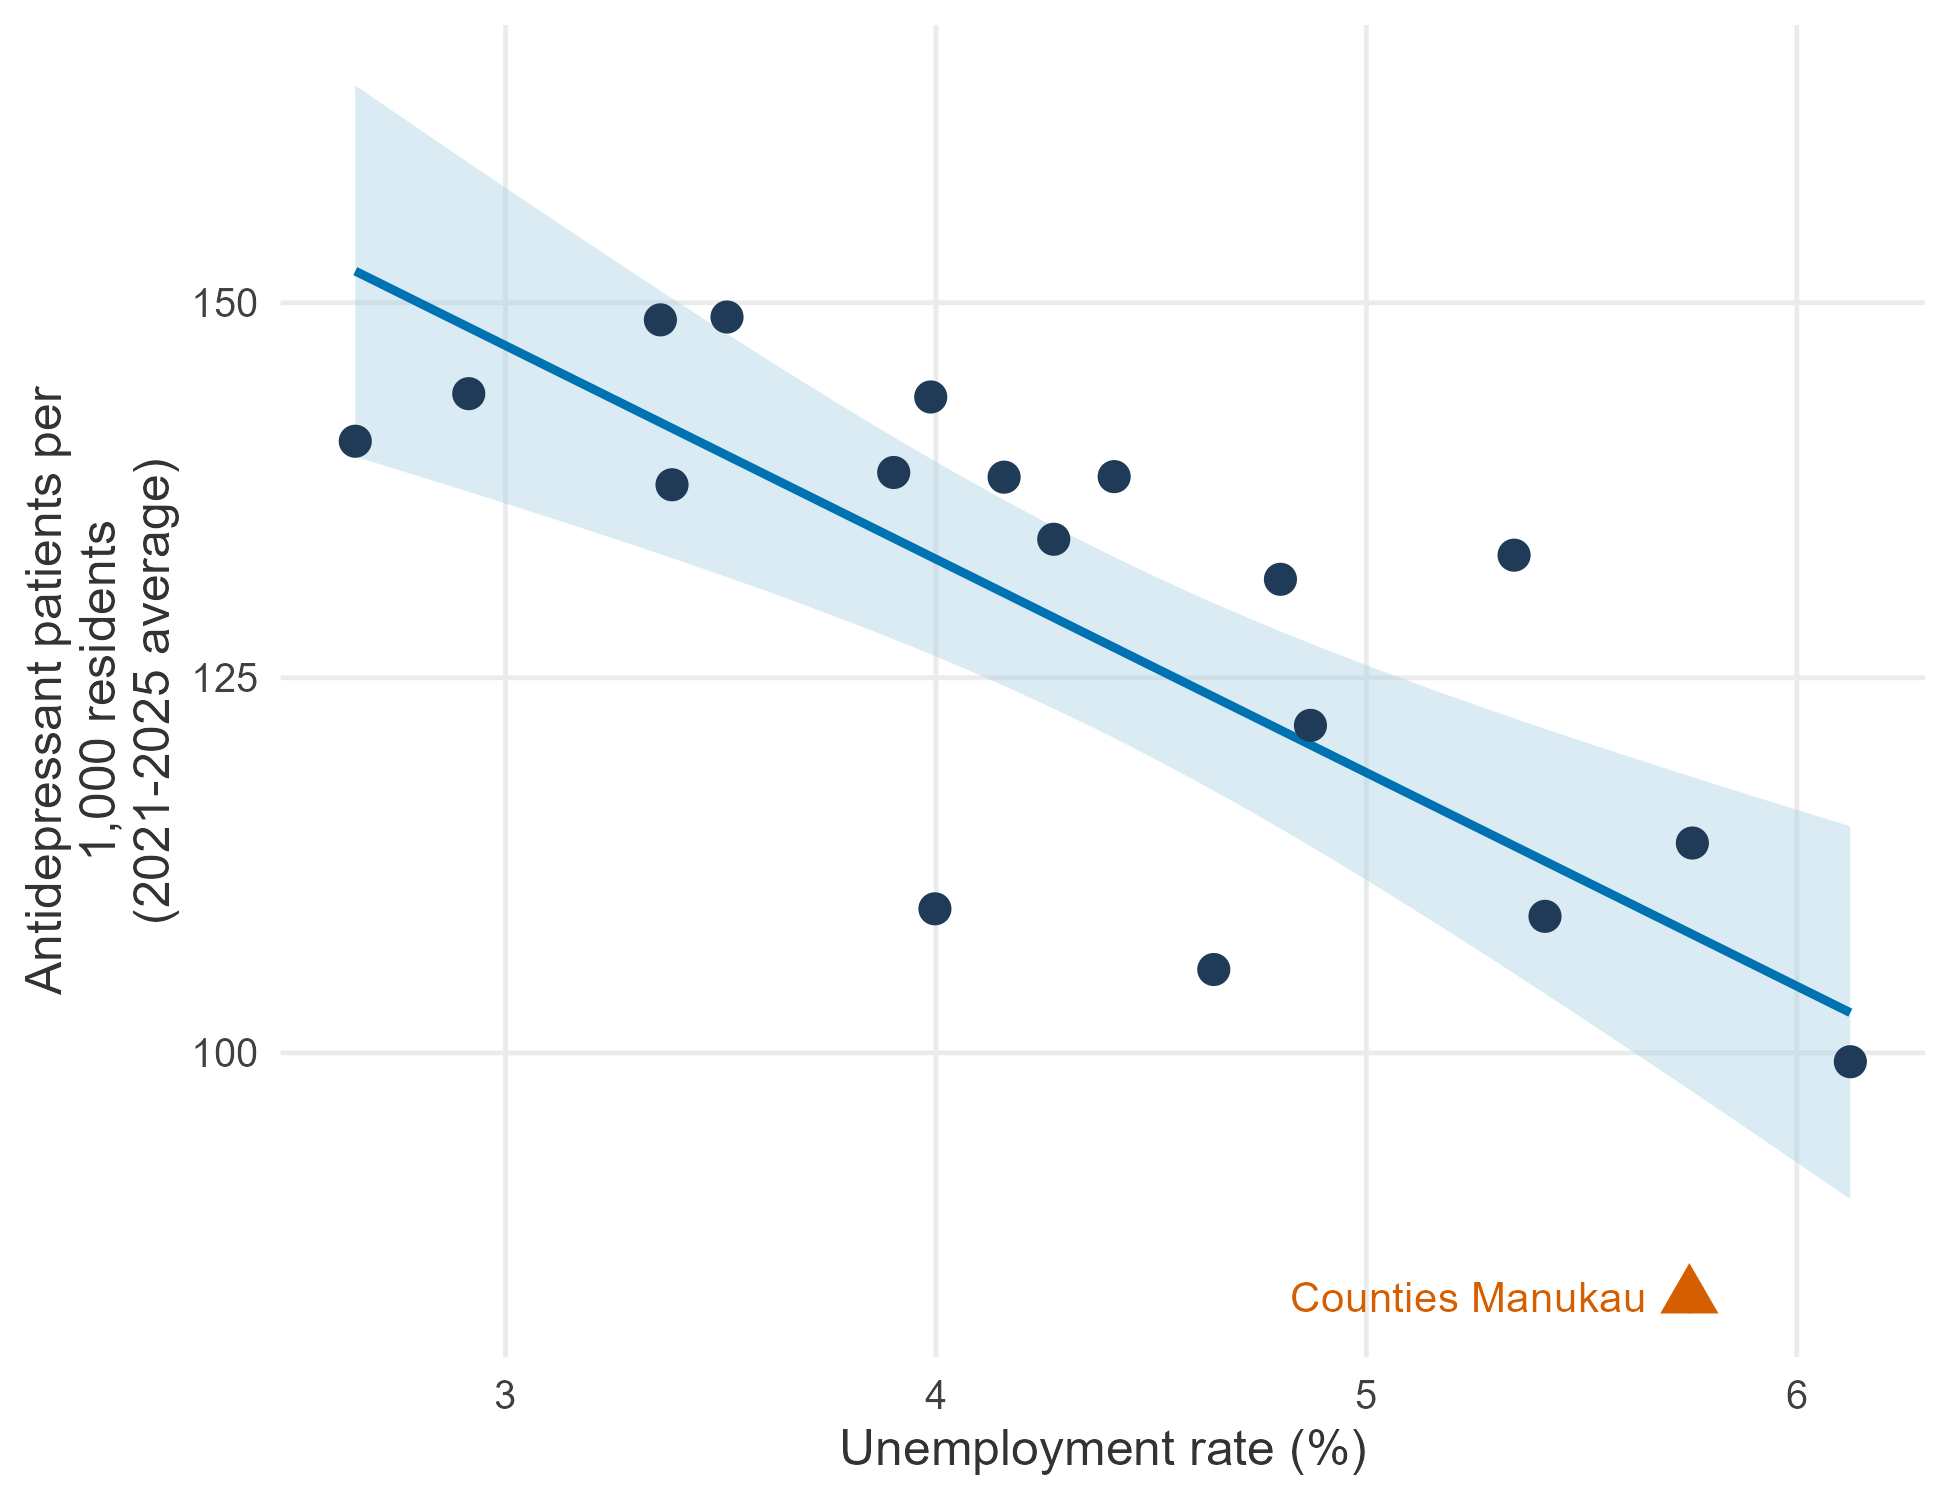
\includegraphics[width=0.7\textwidth]{scatter_unemployment.png}
\caption{Antidepressant patient rate and unemployment rate by district with a fitted line and 95\% confidence band. The triangle marks Counties Manukau.}
\label{fig:scatter}
\end{figure}

% =========================================================
\section{Detailed Analysis Results}

\subsection{Question and hypotheses}
I looked at whether the unemployment rate is linked to the antidepressant patient rate, taking account of age and year, using a two tailed test at the 5\% significance level. The null hypothesis is that the unemployment coefficient is zero.

\subsection{Method}
I used all five years of the data (giving 95 district-year observations ). Each district appears five times with the same Census data so the observations from a given district are not independent. So a linear mixed model deals with this by having a separate starting level and a separate yearly trend for each district. So the model I fitted was one in which the patient rate was a function of the unemployment rate, the \% aged 30-64 and the number of years since 2021, with a random intercept and a random slope for each district. In words:
\begin{quote}
patient rate $=$ intercept $+$ (unemployment effect $\times$ unemployment rate) $+$ (age effect $\times$ percentage aged 30--64) $+$ (year effect $\times$ years since 2021) $+$ a district-specific starting level $+$ a district-specific yearly trend $+$ unexplained variation.
\end{quote}

The coefficients were tested using a $t$-tests. The model was fitted in R-studio using lme4 and lmerTest packages. A likelihood ratio test showed that the model with each district having its own yearly trend fitted the data better than the model where the only difference between districts was in their initial level ($\chi^2 = 51.5$ on 2 df, $p<0.001$). The district trend model was therefore used as the main model.

\subsection{Results}
Table~\ref{tab:model} shows the model estimates. After allowing for age and year, each 1 percentage point increase in the unemployment rate was associated with 12.5 fewer antidepressant patients per 1,000 (95\%  CI 7.3 to 17.7 fewer; $t=-5.11$, df $=16$, $p<0.001$). The null hypothesis was therefore rejected (higher unemployment was associated with lower patient rates). On average patient rates were increasing by 2.3 per 1,000 each year (95\%  CI 1.8 to 2.8). There was quite a bit of variation in the starting levels of the districts (SD 11.2 patients per 1,000) and only a very small amount of variation in the annual trend (SD 1.0 per year) so most of the difference between the districts is in the level of the rates rather than the rate of change.

\begin{table}[H]
\centering
\caption{Mixed model estimates for the antidepressant patient rate (patients per 1,000 residents), 19 districts, 2021-2025.}
\label{tab:model}
\begin{tabular}{lrrrr}
\toprule
\textbf{Term} & \textbf{Estimate} & \textbf{SE} & \textbf{95\% CI} & \textbf{$p$} \\
\midrule
Intercept                       & 410.65   & 76.22 & (249.07, 572.23)    & $<0.001$ \\
Unemployment rate (per 1 point) & $-12.51$ & 2.45  & ($-17.70$, $-7.33$) & $<0.001$ \\
Aged 30--64 (per 1 point)       & $-5.34$  & 1.69  & ($-8.91$, $-1.76$)  & 0.006    \\
Year (per year since 2021)      & 2.32     & 0.24  & (1.82, 2.83)        & $<0.001$ \\
\bottomrule
\end{tabular}

\vspace{0.4em}
{\footnotesize The intercept is the predicted rate at 0\% unemployment and 0\% aged 30-64 in 2021 and is not interpreted. Random effect standard deviations: district starting level 11.2, district yearly trend 1.0, residual 1.0.}
\end{table}

The age estimate statistically significant in this model but not in two of the others in Section~\ref{sec:checks} ($p=0.09$ and $p=0.14$) and the age variable only varies from 42\% to 47\% across the districts. It's therefore a very unstable estimate and I just treat age as a control variable rather than interpret it any further.

\subsection{Checks and sensitivity} \label{sec:checks} 
Table~\ref{tab:sens} shows the estimate of unemployment remains negative under all other modelling assumptions. If you treat each year as a separate step rather than as a straight line trend you get a larger estimate ($-15.1$). A simple linear model with standard errors adjusted for the repeated observations of each district gives the same estimate but with a wider interval. Excluding Counties Manukau (the district with the lowest rate) gives a smaller estimate ($-10.4$, 95\% CI $-15.3$ to $-5.6$, $p<0.001$) so the result is not dependent on that district (although it does pull the estimate down). The estimate across all versions is between 10.4 and 15.1 fewer patients per 1,000 for each percentage point of unemployment.

\begin{table}[H]
\centering
\caption{Estimated change in patients per 1,000 residents for each 1 percentage point increase in unemployment, under different model choices.}
\label{tab:sens}
\begin{tabular}{p{8.4cm}rr}
\toprule
\textbf{Model} & \textbf{Estimate} & \textbf{95\% CI} \\
\midrule
Main model (district specific starting level and trend)           & $-12.51$ & ($-17.70$, $-7.33$) \\
Year as separate steps, district specific starting level          & $-15.11$ & ($-21.09$, $-9.13$) \\
Simple linear model, standard errors adjusted for district        & $-15.11$ & ($-21.63$, $-8.59$) \\
Main model without Counties Manukau                               & $-10.45$ & ($-15.30$, $-5.59$) \\
\bottomrule
\end{tabular}
\end{table}

I also looked at whether the association changed over time, the estimated interaction suggested it may have strengthened slightly each year (-0.47 per 1,000 per year, 95\% CI -0.95 to 0.01, $p=0.055$), although this wasn't statistically significant when allowed the districts to have their own different trends. I don't think we can say the relationship changed.

Figure~\ref{fig:resid} is the plot of residuals against the fitted values for the main model. The residuals are scattered both above and below zero with no noticeable curve, which is as it should be if the straight line relationships in the model are valid. All the residuals are within about 2.5 patients per 1,000 of the fitted rate (which is very small in comparison to the differences between the districts, the average rates ranging from 84 to 149). The spread is a bit wider at the lower fitted rates (around 100 to 120) than at the higher ones. The five largest residuals are from Tair\={a}whiti  ($-2.5$ in 2025 and $+1.9$ in 2023), Lakes ($+1.9$ in 2025 and $+1.8$ in 2021) and Whanganui ($+1.7$ in 2021). The two large residuals from Tair\={a}whiti have opposite signs which suggests that it is simply a case of year on year variation in that district rather than a consistent offset. With only 19 districts we can't be sure whether the uneven spread is due to non constant variance or just chance so the $p$-values should be treated as approximate. The residuals are small in part because the model gives each district its own starting level and trend so this plot says less about the unemployment and age effects than it would for a simple model.

\begin{figure}[H]
\centering
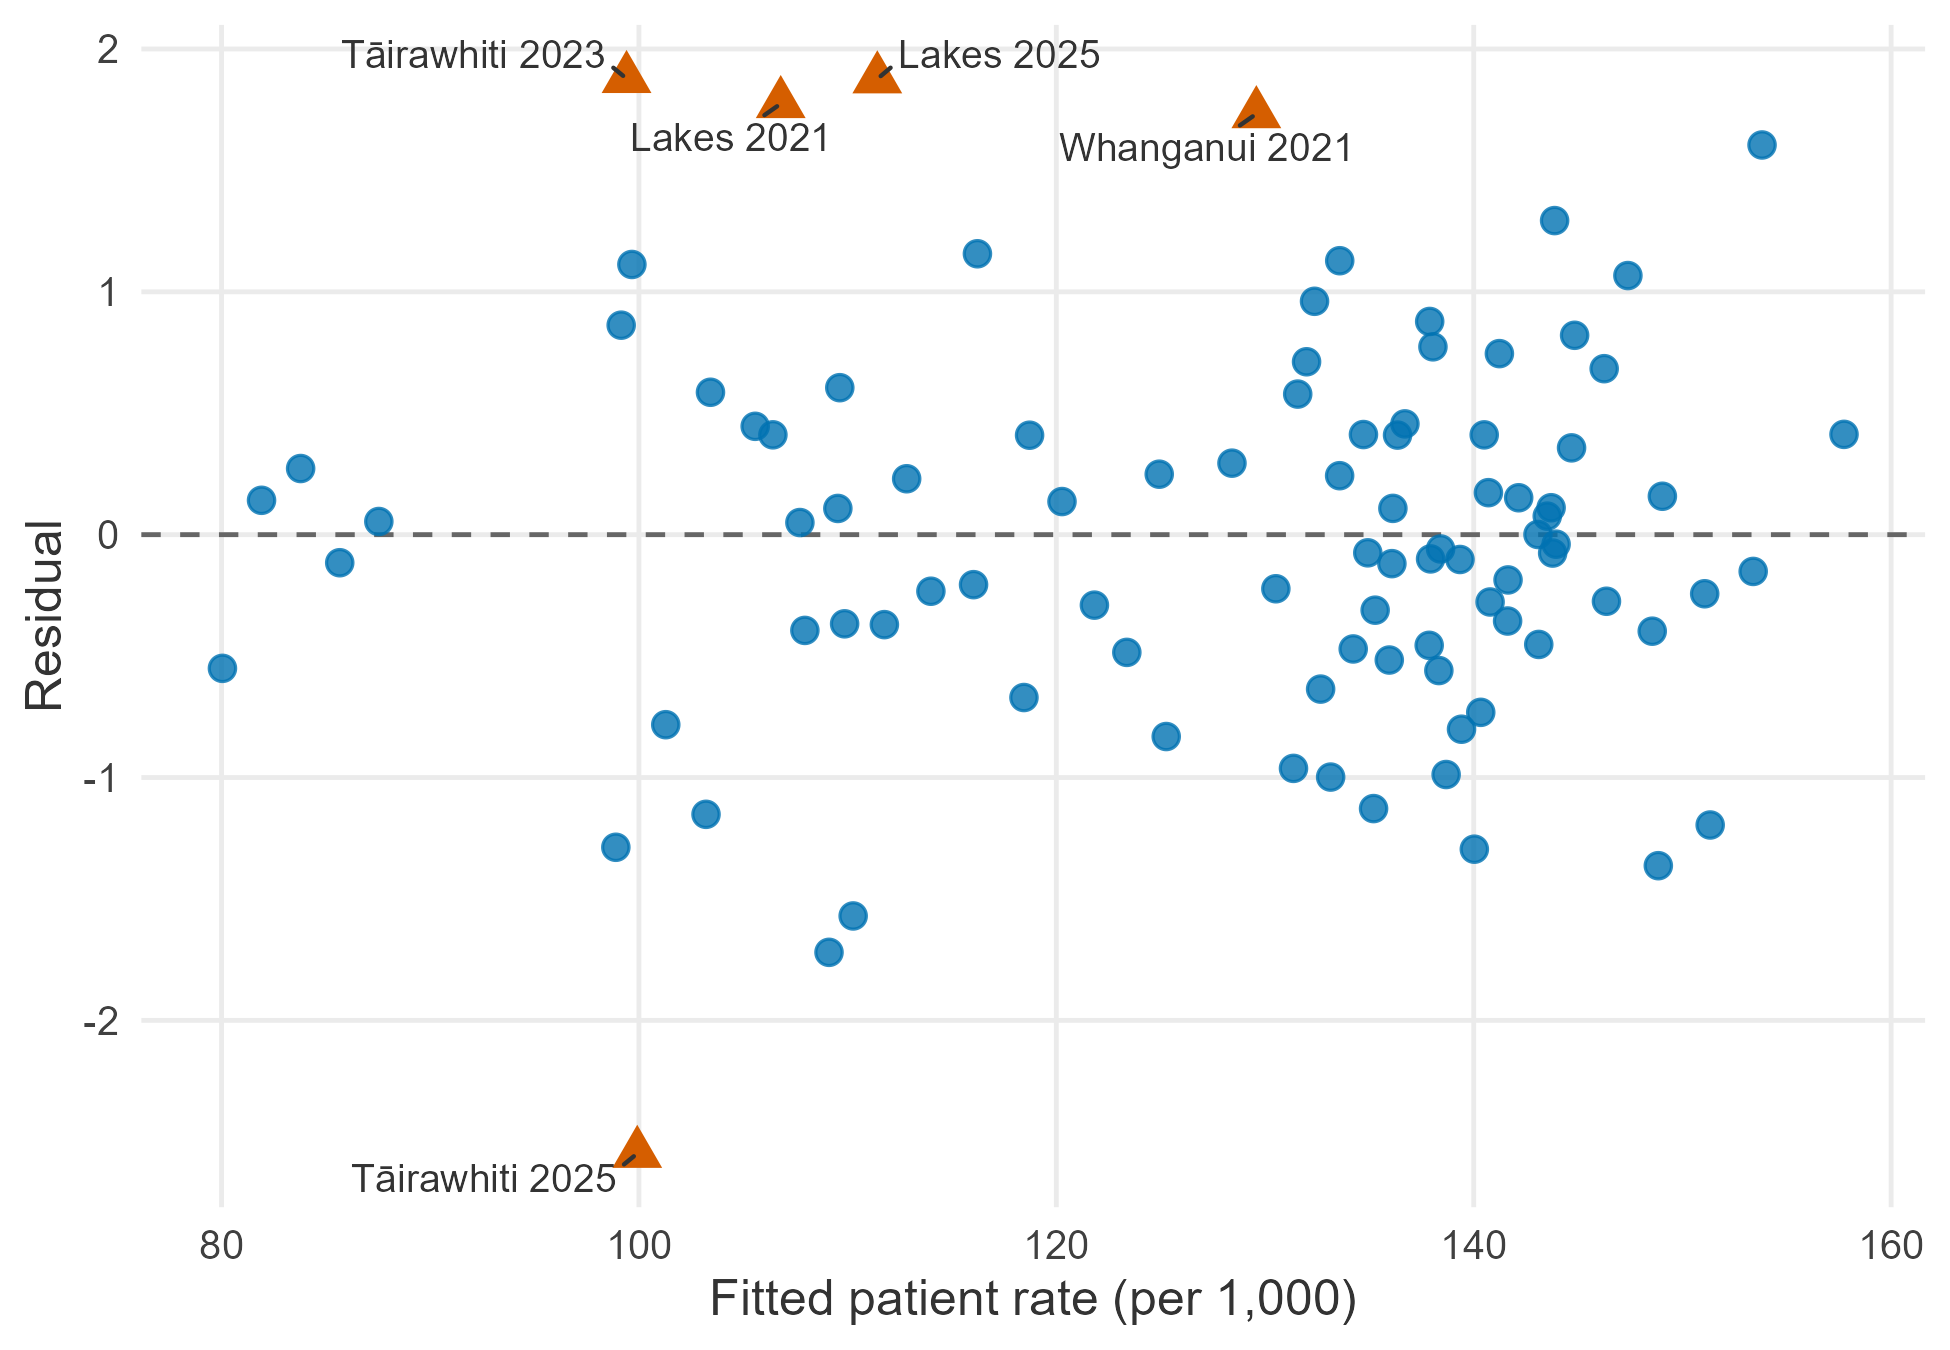
\includegraphics[width=0.7\textwidth]{residuals_mixed.png}
\caption{Residuals against fitted values for the main model. The dashed line marks a residual of zero; triangles mark the five largest residuals.}
\label{fig:resid}
\end{figure}

\subsection{Limitations and possible biases}
Only 19 districts are available so the estimates are very imprecise and the effect of age in particular cannot be separated out with any confidence. The census figures from 2023 were used for all years so the results are describing districts which had higher unemployment in 2023 rather than changes in unemployment over time and population growth is not picked up in the rates. The model assumes a straight line for the year trend which is a very simple assumption with only 5 years of data. The results are describing differences between districts and are not applicable to individuals. The data are only on subsidised dispensings and dispensing is a reflection of access to prescribers and prescribing as well as health need so a lower rate does not imply lower need. The patient counts only include those who had at least one initial dispensing in the year so those who only had repeat dispensions of an existing prescription are not included. The rate is therefore not the proportion of residents taking an antidepressant and could be influenced by the length of time prescriptions last. The therapeutic group doesn't indicate why the drug was prescribed \cite{hnz}. The Capital \& Coast and Hutt Valley figures have been combined so a person who moved between the two districts during the year could be counted twice (though this is likely to be very rare). The model was tweaked as a result of the initial exploratory analysis and the residuals were a little non symmetrical with a few relatively large values so the $p$-values should be treated as approximate.

% =========================================================
\section{Conclusions and Recommendations}

\subsection{Main conclusions}
Districts with higher unemployment had lower antidepressant patient rates. After adjusting for age  and year, each additional percentage point of unemployment was associated with approximately 12.5 fewer patients per 1,000 (95\% CI 7.3 to 17.7, $p<0.001$). The estimate remained clearly negative in all alternative models and when the lowest rate district (Counties Manukau) was removed, ranging from 10.4 to 15.1 fewer patients per 1,000. On average patient rates increased by around 2.3 patients per 1,000 each year between 2021 and 2025 (95\% CI 1.8 to 2.8) and they increased in both the high and low unemployment groups of districts. The high unemployment group remained lower in every year. An exploratory test suggested the gap may have widened slightly over time, though this was not statistically significant ($p=0.055$) and I don't claim that the relationship has changed.

\subsection{What the results do and don't show}
The results describe differences between districts, they do not indicate that unemployment leads to reduced use of antidepressants and should not be interpreted as suggesting lower levels of mental health need in the higher unemployment districts. Prescribing is influenced by access to prescribers, by how conditions are diagnosed and by prescribing practice as much as by need so it's quite possible that access varies between districts (though this analysis is not designed to test that).

\subsection{Recommendations}
Health planners should be careful about low dispensing rates and should not use them in isolation as an indicator of need. It would be sensible to look at whether access to both GP and mental health services differs between areas of higher and lower unemployment before making any judgements about need. Any such work should report rates per 1,000 rather than raw numbers (the numbers would be skewed by the size of the district) and should be wary of any deficit based interpretation of any community.

\subsection{Limitations}
The principal constraints are the small number of districts (19), the use of 2023 Census figures for all five years and the district level of the data. The model employed a simple linear year trend and the residuals were broadly even with a few relatively large values (Section~\ref{sec:checks}) so the p-values should be regarded as approximate. The age estimate was very unstable across the models and should not be interpreted.

\subsection{Future work}
Future work could incorporate annual local unemployment data to allow study of the time series of unemployment, add in other district characteristics (ethnic composition, deprivation, access to GP etc) and compare with other medicine groups. A longer time series would also allow for a more detailed mixed model with year level effects.

\newpage
% =========================================================
\begin{thebibliography}{9}
\bibitem{lme4} Bates, D., M\"achler, M., Bolker, B., \& Walker, S. (2015). Fitting linear mixed-effects models using lme4. \textit{Journal of Statistical Software}, 67(1), 1--48.
\bibitem{hnz} Health New Zealand. (2026). \textit{Pharmaceutical Data web tool}, version 07 August 2026. Data extracted from the Pharmaceutical Collection on 09 July 2026.
\bibitem{lmertest} Kuznetsova, A., Brockhoff, P. B., \& Christensen, R. H. B. (2017). lmerTest package: Tests in linear mixed effects models. \textit{Journal of Statistical Software}, 82(13), 1--26.
\bibitem{paeora} Ministry of Health NZ. (2022). \textit{Healthy Futures (Pae Ora) Act 2022}.
\bibitem{R} R Core Team. (2025). \textit{R: A language and environment for statistical computing}. R Foundation for Statistical Computing.
\bibitem{census} Stats NZ. (2023). \textit{Aotearoa Data Explorer: 2023 Census, Totals by Topic}.
\bibitem{mh} Yang, Y., Niu, L., Amin, S., \& Yasin, I. (2024).
\textit{Unemployment and mental health: A global study of
unemployment's influence on diverse mental disorders.}

\end{thebibliography}

\end{document}